\documentclass[hyperref=unicode, aspectratio=169]{beamer}
\usepackage[utf8]{inputenc}
\usepackage[T2A]{fontenc}
\usepackage[russian]{babel}
\usepackage[backend=biber]{biblatex}
\usepackage{csquotes}
\usepackage{tikzit}
\usepackage{mathabx}
\usepackage{bookmark}
\usepackage{makecell}

\title{Построение многопроцессорного расписания с использованием жадных стратегий и ограниченного перебора}
\usetheme{Antibes}
\author{Савицкий Илья\\Научный руководитель: к.т.н. доцент Костенко Валерий Алексеевич}
\date{19 апреля 2022 г.}
\logo{
\includegraphics[width=1.5cm]{imgs/asvk-logo.png}}

\addbibresource{biblio.bib}

\definecolor{ASVKaccent}{rgb}{0.20392,0.02745,0.34509}
\usecolortheme[named=ASVKaccent]{structure}

\input{block-schemas.tikzstyles}

\begin{document}
\begin{frame}
    \titlepage
\end{frame}

\begin{frame}
    \tableofcontents
\end{frame}

\section{Постановка задачи}
\subsection{Определения}

\begin{frame}
    \frametitle{Постановка задачи}
    \begin{columns}
        \begin{column}{0.6\textwidth}
            Дано:
            \begin{enumerate}
                \item Ориентированный граф работ $G$ без циклов, в котором дуги - зависимости по данным, а вершины - задания. Вершин $n$, дуг $m$
                \item Вычислительная система, состоящая из $p$ различных процессоров
                \item Матрица $C_{ij}$ длительности выполнения работ на процессорах, $i=1 \dots n, j=1 \dots p$
                \item Матрица $D_{kl}$ передач данных между процессорами, $k=1 \dots p, l = 1 \dots p, D_{kk} = 0$
            \end{enumerate}
        \end{column}
        \begin{column}{0.4\textwidth}
            \ctikzfig{graph_schema}
        \end{column}
    \end{columns}
\end{frame}

\begin{frame}
    \frametitle{Постановка задачи}
    \begin{columns}
        \begin{column}{0.6\textwidth}
            Требуется:
            \begin{enumerate}
                \item Построить расписание $HP$, то есть для каждой работы определить время начала ее выполнения и процессор на которм она будет выполняться
                \item Минимизируемый критерий: время завершения выполнения расписания
                \item Дополнительные ограничения
            \end{enumerate}
        \end{column}
        \begin{column}{0.4\textwidth}
            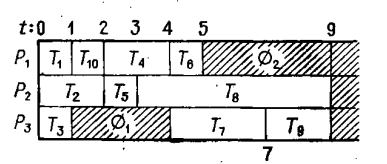
\includegraphics[width=\textwidth]{imgs/schedule.png}
        \end{column}
    \end{columns}
    % \footfullcite{coffman1976}
\end{frame}

\begin{frame}
    \frametitle{Модель расписания}
    Множество корректных расписаний $HP$ задается набором ограничений:
    \begin{itemize}
        \item В расписании не допустимы прерывания
        \item Интервалы выполнения заявок не пересекаются
        \item Каждая работа назначена на процессор
        \item Любую работу обслуживает один процессор
    \end{itemize}
\end{frame}

\begin{frame}
    \frametitle{Постановки задачи}
    \begin{enumerate}
        \item Задача с однородными процессорами (длительность выполнения работы не зависит от того, на каком процессоре она выполняется) и дополнительными ограничениями на количество передач:
        \begin{itemize}
            \item $CR = \frac{m_{ip}}{m}$ - количество передач данных между работами на каждый процессор
            \item $CR2 = \frac{m_{2_edg}}{m}$ - количество дуг, начальный и конечный узлы которых назначены на процессоры, не соединенных напрямую
        \end{itemize}
        \item Задача с однородными процессорами и контролем сбалансированности распределения работ:
        \begin{itemize}
            \item $BF = \left( \frac{a_{max} \cdot p}{n} \right)$ - наибольшее, по всем процессорам, количество работ на процессоре
        \end{itemize}
        \item Задача с неоднородными процессорами, но без дополнительных ограничений на расписание
    \end{enumerate}
\end{frame}



\section{Описание алгоритма}
% \begin{frame}
%     \frametitle{Существующие алгоритмы}
%     {
%         \small
%         \begin{tabular}{| c | c | c | c | }
%             \hline
%             \makecell{Название          \\алгоритма} & Рандомизированность & Итерационный & \makecell{Возможность \\ масштабирования} \\
%             \hline
%             \makecell{Генетические      \\алгоритмы} & Рандомный & Итерационный & +/- \\
%             \hline
%             \makecell{Алгоритм имитации \\отжига} & Рандомный & Итерационный & + \\
%             \hline
%             \makecell{Муравьиные        \\алгоритмы} & Рандомный & Итерационный & - \\
%             \hline
%             \makecell{Жадные стратегии  \\и ограниченный перебор} & Рандомный & Конструктивный & + \\
%             \hline
%         \end{tabular}
%     }
% \end{frame}
\subsection{Схема}
\begin{frame}
    \frametitle{Общая схема жадного алгоритма}
    {\tiny
        \ctikzfig{algo_schema}
    }
\end{frame}

\subsection{Предподсчет}

\begin{frame}
    \frametitle{Блок-схема предподсчета}
    {\tiny
        \ctikzfig{precalc}
    }
    % \ctikzfig{precalc}
\end{frame}

\begin{frame}
    \frametitle{Предподсчет}
    \begin{columns}
        \begin{column}{0.6\textwidth}
            \begin{enumerate}
                \item Формируется множество $D=d_1, d_2, \dots, d_l$, где $l$ - количество вершин, доступных для добавления(т.е. у которых нет предшественников в исходном графе)
                \item Вычисляется вектор $k$ - вектор длин критических путей от "головной" вершины до каждой вершины графа. В случае, если такой вершины нет - создается фиктивная вершина с нулевой длительностью. Вектор $k$ заполняется при помощи алгоритма Дейкстры.
            \end{enumerate}
        \end{column}
        \begin{column}{0.4\textwidth}
            \ctikzfig{fictive_nodes}
        \end{column}
    \end{columns}
\end{frame}


\subsection{Пробное размещение работы}
\begin{frame}
    \frametitle{Блок-схема пробного размещения работы}
    {\tiny
        \ctikzfig{choosing}
    }
\end{frame}

\begin{frame}
    \frametitle{Жадный критерий выбора размещения}
    Из множества $D$(выделено красным) выбирается работу по критерию максимальности количества потомков у вершины.
    \ctikzfig{max_children}
    
\end{frame}

\begin{frame}
    \frametitle{Пробное размещение работы}
    Пробное размещение работы производится с учетом  жадного и дополнительных критериев. \\
    Жадный критерий - скорейшее завершение работы в расписании. \\
    Способы выбора места:
    \begin{enumerate}
        \item Подсчет усредненного взвешенного показателя среди критериев \\
              \begin{gather*}
                  crit = C_1 \cdot GR + C_2 \cdot CR + C_3 \cdot BF
              \end{gather*}
              ,где $GR$ - время скорейшего завершения работы, $C_1, C_2, C_3$ - параметры алгоритма
        \item Допускная система с выбором
    \end{enumerate}
\end{frame}

\begin{frame}
    \frametitle{Допускная система выбора}
    \begin{enumerate}
        \item Список мест размещения работ ранжируется по $GR$, после чего отсекаются верхние $n\%$ работ
        \item Такие же действия повторяются для каждого дополнительного критерия
        \item В конечном списке выбрать место по жадному критерию
    \end{enumerate}
    ,где $n$ - параметр алгоритма
\end{frame}


\subsection{Ограниченный перебор}
\begin{frame}
    \frametitle{Процедура ограниченного перебора}
    После неудачной пробной постановки работы в расписание алгоритм создает набор $K=k_1,k_2,\dots,k_t$, состоящий из $t$ последних добавленных работ ($t$ – параметр алгоритма). Далее, процедурой полного перебора пробуются различные расписания до тех пор, пока не получится расписание, удовлетворяющее критерию критичности пути до последней поставленной работы и удовлетворяющее дополнительные критерии
\end{frame}

\subsection{Корректировка критичности пути}
\begin{frame}
    \frametitle{Блок схема корректировки расписания}
    {\tiny
        \ctikzfig{criticalness}
    }
\end{frame}

\section{Текущие результаты}
\begin{frame}
    \frametitle{Текущие результаты}
    \begin{enumerate}
        \item Проведен обзор алгоритмов построения списочных расписаний. Цель обзора; выявление жадных критериев и схем ограниченного перебора которые могут быть модифицированы для решения данной задачи.
        \item Разработан и реализован алгоритм
        \vspace{0.3cm}
        \hrule
        \vspace{0.2cm}
        \item Проведено исследование свойств алгоритма на данных от Хуавей.
    \end{enumerate}
\end{frame}

\end{document}